% Created 2022-04-17 Sun 14:58
% Intended LaTeX compiler: pdflatex
\documentclass[11pt]{article}
\usepackage[utf8]{inputenc}
\usepackage[T1]{fontenc}
\usepackage{graphicx}
\usepackage{longtable}
\usepackage{wrapfig}
\usepackage{rotating}
\usepackage[normalem]{ulem}
\usepackage{amsmath}
\usepackage{amssymb}
\usepackage{capt-of}
\usepackage{hyperref}
\graphicspath{{../../books/}}
% TIPS
% \substack{a\\b} for multiple lines text





% pdfplots will load xolor automatically without option
\usepackage[dvipsnames]{xcolor}

\usepackage{forest}
% two-line text in node by [two \\ lines]
% \begin{forest} qtree, [..] \end{forest}
\forestset{
  qtree/.style={
    baseline,
    for tree={
      parent anchor=south,
      child anchor=north,
      align=center,
      inner sep=1pt,
    }}}
%\usepackage{flexisym}
% load order of mathtools and mathabx, otherwise conflict overbrace

\usepackage{mathtools}
%\usepackage{fourier}
\usepackage{pgfplots}
\usepackage{amsthm, mathabx,  amsmath, commath}
\usepackage{amsfonts}

\usepackage{empheq}
\usepackage{tikz}
\usetikzlibrary{arrows.meta}
\usepackage[most]{tcolorbox}

\newtheorem{theorem}{Theorem}[section]
\newtheorem{definition}{Definition}[section]
\newtheorem{corollary}{Corollary}[section]
\newtheorem{example}{Example}[section]
\newtheorem{lemma}{Lemma}[section]
\newtheorem{proposition}{Proposition}[section]

\newcommand{\bl}[1] {\boldsymbol{#1}}
\newcommand{\Wt}[1] {\stackrel{\sim}{\smash{#1}\rule{0pt}{1.1ex}}}
\newcommand{\wt}[1] {\widetilde{#1}}


%For boxed texts in align, use Aboxed{}
%otherwise use boxed{}

\DeclareMathSymbol{\widehatsym}{\mathord}{largesymbols}{"62}
\newcommand\lowerwidehatsym{%
  \text{\smash{\raisebox{-1.3ex}{%
    $\widehatsym$}}}}
\newcommand\fixwidehat[1]{%
  \mathchoice
    {\accentset{\displaystyle\lowerwidehatsym}{#1}}
    {\accentset{\textstyle\lowerwidehatsym}{#1}}
    {\accentset{\scriptstyle\lowerwidehatsym}{#1}}
    {\accentset{\scriptscriptstyle\lowerwidehatsym}{#1}}
}

\usepackage{graphicx}
    
% text on arrow for xRightarrow
\makeatletter
%\newcommand{\xRightarrow}[2][]{\ext@arrow 0359\Rightarrowfill@{#1}{#2}}
\makeatother


\def \bx {\boldsymbol{x}}
\def \ba {\boldsymbol{a}}
\def \bI {\boldsymbol{I}}
\def \bt {\boldsymbol{t}}
\def \bb {\boldsymbol{b}}
\def \bA {\boldsymbol{A}}
\def \bX {\boldsymbol{X}}
\def \bu {\boldsymbol{u}}
\def \bS {\boldsymbol{S}}
\def \bZ {\boldsymbol{Z}}
\def \bz {\boldsymbol{z}}
\def \by {\boldsymbol{y}}
\def \bw {\boldsymbol{w}}
\def \bT {\boldsymbol{T}}
\def \bS {\boldsymbol{S}}
\def \bm {\boldsymbol{m}}
\def \bW {\boldsymbol{W}}
\def \bY {\boldsymbol{Y}}
\def \bH {\boldsymbol{H}}
\def \blambda {\boldsymbol{\lambda}}
\def \bPhi {\boldsymbol{\Phi}}
\def \btheta {\boldsymbol{\theta}}
\def \bmu {\boldsymbol{\mu}}
\def \bphi {\boldsymbol{\phi}}
\def \bSigma {\boldsymbol{\Sigma}}
\def \lb {\left\{}
\def \rb {\right\}}
\def \caln {\mathcal{N}}
\def \dissum {\displaystyle\Sigma}
\def \dispro {\displaystyle\prod}
\def \E {\mathbb{E}}
\def \Q {\mathbb{Q}}
\def \V {\mathbb{V}}
\def \R {\mathbb{R}}
\def \calq {\mathcal{Q}}
\def \calg {\mathcal{G}}
\def \caln {\mathcal{N}}
\def \calr {\mathcal{R}}
\def \calm {\mathcal{M}}
\def \calc {\mathcal{C}}
\def \bcup {\bigcup}

\DeclareMathOperator{\use}{\textsf{use}}
\DeclareMathOperator{\Cop}{Cop}
\DeclareMathOperator{\non}{\textsf{non}}
\makeindex
\author{Andre Nies}
\date{\today}
\title{Computability and Randomness}
\hypersetup{
 pdfauthor={Andre Nies},
 pdftitle={Computability and Randomness},
 pdfkeywords={},
 pdfsubject={},
 pdfcreator={Emacs 28.0.92 (Org mode 9.6)}, 
 pdflang={English}}
\begin{document}

\maketitle
\tableofcontents


\section{The complexity of sets}
\label{sec:orgfcef0e4}
\subsection{The basic concepts}
\label{sec:org32b3157}
\subsubsection{Partial computable functions}
\label{sec:org5e53717}
Given expression \(\alpha\), \(\beta\),
\begin{equation*}
\alpha\simeq\beta
\end{equation*}
means that either both expressions are undefined, or they are defined with the same value

The function \(\Xi(e,x)\simeq\Phi_e(x)\). A Turing program computing \(\Xi\) is called a \textbf{universal Turing program}

\begin{theorem}[Parameter Theorem]
For each partial computable function \(\Theta\) in two variables there is a computable strictly
increasing function \(q\) s.t.
\begin{equation*}
\forall e\forall x\Phi_{q(e)}(x)\simeq\Theta(e,x)
\end{equation*}
An index for \(q\) can be obtained effectively from an index for \(\Theta\)
\end{theorem}

\begin{lemma}[Padding Lemma]
For each \(e\) and each \(m\), one may effectively obtain \(e'>m\) s.t. the Turing
program \(P_{e'}\) behaves exactly like \(P_e\)
\end{lemma}

\begin{theorem}[Recursion Theorem]
\label{1.1.5}
Let \(g:\N\to\N\) be computable. Then there is an \(e\) s.t. \(\Phi_{g(e)}=\Phi_e\). We say that \(e\) is a
\textbf{fixed point} for \(g\)
\end{theorem}

\begin{proof}
There is \(q\) s.t. \(\Phi_{q(e)}(x)\simeq\Phi_{g(\Phi_e(e))}(x)\) for all \(e,x\). Choose an \(i\)
s.t. \(q=\Phi_i\), then
\begin{equation*}
\Phi_{q(i)}=\Phi_{\Phi_i(i)}=\Phi_{g(\Phi_i(i))}
\end{equation*}
\end{proof}

\begin{theorem}[Recursion Theorem with Parameters]
\label{1.1.6}
Let \(g:\N^2\to\N\) be computable. Then there is a computable function \(f\), which can be obtained
effectively from \(g\), s.t. \(\Phi_{g(f(n),n)}=\Phi_{f(n)}\) for each \(n\)
\end{theorem}

\begin{proof}
There is \(g_n\) s.t. \(g_n(f(n))=g(f(n),n)\). Then let \(f(n)\) be the fixed point of \(\Phi_{g'(x)}\)
\end{proof}

\begin{exercise}
\label{1.1.7}
Extend the Recursion Theorem by showing that computable function \(g\) has infinitely many fixed
points. Conclude that the function \(f\) in Theorem \ref{1.1.6} can be chosen one-one
\end{exercise}

\begin{proof}
There is infinite many \(i\) s.t. \(q=\Phi_i\)
\end{proof}
\subsubsection{Computably enumerable sets}
\label{sec:org5e81737}
\begin{definition}[]
\(A\subseteq\N\) is \textbf{computably enumerable} (\textbf{c.e.}) if \(A\) is the domain of some partial computable function
\end{definition}

Let
\begin{equation*}
W_e=\dom(\Phi_e)
\end{equation*}
Then \((W_e)_{e\in\N}\) is an effective listing of all c.e. sets. A sequence of sets \((S_e)_{e\in\N}\)
s.t. \(\{\la e,x\ra:x\in S_e\}\) is c.e. is called \textbf{uniformly computably enumerable}

\(A\) is called \textbf{computable} if its characteristic function is computable; otherwise \(A\) is
called \textbf{incomputable}

\begin{proposition}[]
\(A\) is computable \(\Leftrightarrow\) \(A\) and \(\N-A\) are c.e.
\end{proposition}

We may obtain a c.e. incomputable set denoted \(\emptyset'\) by a direct diagonalization. We
define \(\emptyset'\) in such a way that \(\N-\emptyset'\) differs from \(W_e\) at \(e\): let
\begin{equation*}
\emptyset'=\{e:e\in W_e\}
\end{equation*}
The set \(\emptyset'\) is called the \textbf{halting problem}, since \(e\in\emptyset'\) iff program \(P_e^1\) halts on input \(e\)

\begin{proposition}[]
The set \(\emptyset'\) is c.e. but not computable
\end{proposition}

\begin{proof}
\(\emptyset'\) is c.e. since \(\emptyset'=\dom(J)\), where \(J\) is the partial computable function given
by \(J(e)\simeq\Phi_e(e)\). If \(\emptyset'\) is computable then there is \(e\) s.t. \(\N-\emptyset'=W_e\).
Then \(e\in\emptyset'\leftrightarrow e\in W_e\leftrightarrow e\in\emptyset'\), a contradiction
\end{proof}

The sequence \((W_e)_{e\in\N}\) is universal for uniformly c.e. sequences

\begin{corollary}[]
For each uniformly c.e. sequence \((A_e)_{e\in\N}\) there is a computable function \(q\)
s.t. \(A_e=W_{q(e)}\) for each \(e\)
\end{corollary}

\begin{proof}
Define the partial computable function \(\Theta\) by \(\Theta(e,x)\simeq 0\) iff \(x\in A_e\), and \(\Theta(e,x)\) is
undefined otherwise. Then the function \(q\) obtained by the Parameter Theorem is as required.
\end{proof}

\begin{exercise}
\label{1.1.12}
Suppose \((\hatW_e)_{e\in\N}\) is a further universal uniformly c.e. sequence. Assume
that \((\hatW_e)_{e\in\N}\) also has the padding property, one may effectively obtain \(e'>m\)
s.t. \(\hatW_e'=\hatW_e\). Show that there is a computable permutation \(\pi\) of \(\N\)
s.t. \(\hatW_e=W_{\pi(e)}\) for each \(e\)
\end{exercise}

\begin{proof}
there is \(q\) s.t. \(W_{q(e)}=\hatW_e\), there is \(p\) s.t. \(\hatW_{p(e)}=W_e\)
Find
\begin{enumerate}
\item \(q'(e)>e\)
\item \(q'\) is 1-1
\item \(W_{q'(e)}=\hatW_e\)
\end{enumerate}


padding \(\pi(m,e)>m\). \(W_{\pi(e,q(e))}=W_{q(e)}\)

similar to cantor-bernstein

or back-and-forth
\end{proof}
\subsubsection{Indices and approximations}
\label{sec:org7762b60}
\begin{definition}[]
We write
\begin{equation*}
\Phi_{e,s}(x)=y
\end{equation*}
if \(e,x,y<s\) and the computation of program \(P_e\) on input \(x\) yields \(y\) in at
most \(s\) computation steps. Let \(W_{e,s}=\dom(\Phi_{e,s})\)
\end{definition}

At stage \(s\) we have complete information about \(\Phi_{e,s}\) and \(W_{e,s}\). To state this
more formally, we need to specify an effective listing \(D_0,D_1,\dots\) of the finite subsets of \(\N\)

\begin{definition}[]
Let \(D_0=\emptyset\). If \(n>0\) has the form \(2^{x_1}+\dots+2^{x_r}\), where \(x_1<\dots<x_r\), then
let \(D_n=\{x_1,\dots,x_r\}\). We say that \(n\) is a \textbf{strong index} for \(D_n\). For instance, \(D_5=\{0,2\}\)
\end{definition}

There is a computable function \(f\) s.t. \(f(e,s)\) is a strong index for \(W_{e,s}\). We think
of a computable enumeration of a set \(A\) as an effective listing \(a_0,a_1,\dots\) of the elements
of \(A\) in some order. To include the case that \(A\) is finite, we formalize this via an
effective union of finite sets \((A_s)\). We view \(A_s\) as the set of elements enumerated by
the end of stage \(s\). At certain stages we may decide not to enumerate any element

\begin{definition}[]
A \textbf{computable enumeration} of a set \(A\) is an effective sequence \((A_s)_{s\in\N}\) of (strong
indices for) finite sets s.t. \(A_s\subseteq A_{s+1}\) for each \(s\) and \(A=\bigcup_sA_s\)
\end{definition}

Each c.e. set \(W_e\) has the computable enumeration \((W_{e,s})_{s\in\N}\). Conversely, if \(A\)
has a computable enumeration then \(A\) is c.e., for \(A=\dom(\Phi)\) where \(\Phi\) is the partial
computable function given by the following procedure: at stage \(s\) we let \(\Phi(x)=0\)
if \(x\in A_s\). An \textbf{index for a c.e. set} \(A\) is a number \(e\) s.t. \(A=W_e\)

\begin{proposition}[]
For each computable function \(\Phi\), \(\ran(\Phi)\) is c.e.
\end{proposition}

\begin{proof}
Suppose \(\Phi=\Phi_e\) and we enumerate \(A=\ran(\Phi)\). Since we have complete information
about \(\Phi_s\) at stage \(s\), we can compute from \(s\) a strong index for \(A_s=\ran(\Phi_s)\).
Then \((A_s)_{s\in\N}\) is the required computable enumeration of \(A\)
\end{proof}

\begin{exercise}
\label{1.1.17}
\end{exercise}

\begin{exercise}
\label{1.1.19}
\end{exercise}

\begin{proof}
find a subsequence with increasing required steps
\end{proof}
\subsection{Relative computational complexity of sets}
\label{sec:orgc2c59b5}


\begin{definition}[]
\(X\) is \textbf{many-one reducible} to \(Y\), denoted \(X\le_mY\), if there is a computable function \(f\)
s.t. \(n\in X\leftrightarrow f(n)\in Y\) for all \(n\)
\end{definition}

If \(X\) is computable, \(Y\neq\emptyset\), and \(Y\neq\N\), then \(X\le_mY\): choose \(y_0\in Y\) and \(y_1\notin Y\).
Let \(f(n)=y_0\) if \(n\in X\) and \(f(n)=y_1\) otherwise. Then \(X\le_mY\) via \(f\).

For each set \(Y\) the class \(\{X:X\le_mY\}\) is countable. In particular, there is no greatest
many-one degree

\begin{proposition}[]
\label{1.2.2}
\(A\) is c.e. \(\Leftrightarrow\) \(A\le_m\emptyset'\)

An index for the many-one reduction as a computable function can be obtained effectively from a
c.e. index for \(A\), and conversely
\end{proposition}

\begin{proof}
\(\Rightarrow\): We claim that there is a computable function \(g\) s.t.
\begin{equation*}
W_{g(e,n)}=
\begin{cases}
\{e\}&n\in A\\
\emptyset
\end{cases}
\end{equation*}
For let \(\Theta(e,n,x)\) converge if \(x=e\) and \(n\in A\). Then there is a computable function \(g\)
s.t. \(\forall e,n,x[\Theta(e,n,x)\simeq\Phi_{g(e,n)}(x)]\). By Theorem \ref{1.1.6}, there is a computable
function \(h\) s.t. \(W_{g(h(n),n)}=W_{h(n)}\) for each \(n\). Then
\begin{align*}
&n\in A\Rightarrow W_{h(n)}=\{h(n)\}\Rightarrow h(n)\in\emptyset'\\
&n\notin A\Rightarrow W_{h(n)}=\emptyset\Rightarrow h(n)\notin\emptyset
\end{align*}
\(\Leftarrow\): If \(A\le_m\emptyset'\) via \(h\), then \(A=\dom(\Psi)\) where \(\Psi(x)\simeq J(h(x))\) (recall
that \(J(e)\simeq\Phi_e(e)\))
\end{proof}

\begin{definition}[]
A c.e. set \(C\) is called \textbf{\(r\)-complete} if \(A\le_rC\) for each c.e. set \(A\)
\end{definition}

we say that \(X\le_1Y\) if \(X\le_mY\) via a one-one function \(f\)

\begin{exercise}
\label{1.2.4}
The set \(\emptyset'\) is \(1\)-complete
\end{exercise}

\begin{exercise}
\label{1.2.5}
\(X\equiv_1 Y\Leftrightarrow\) there is a computable permutation \(p\) of \(\N\) s.t. \(Y=p(X)\)
\end{exercise}

Our intuitive understanding of ``\(Y\) is at least as complex as \(X\)'' is: \(X\) can be computed
with the help of \(Y\). To formalize more general ways of relative computation, we extend the
machine model by a one-way infinite ``oracle'' tape which holds all the answers to oracle
questions of the form ``is \(k\) in \(Y\)''.

We write \(\Phi_e^Y(n)\downarrow\) if the program \(P_e\) halts when the oracle is \(Y\) and the input
is \(n\); we write \(\Phi_e(Y;n)\) or \(\Phi_e^Y(n)\) for this output. The \(\Phi_e\) are called \textbf{Turing
functionals}. And we let \(W_e^Y=\dom(\Phi_e^Y)\). \(W_e\) is a \textbf{c.e. operator}

\begin{definition}[]
A total function \(f:\N\to\N\) is called \textbf{Turing reducible} to \(Y\), or \textbf{computable relative to} \(Y\),
or \textbf{computable in} \(Y\), if there is an \(e\) s.t. \(f=\Phi_e^Y\). We denote this by \(f\le_TY\). We
also say that \(Y\) \textbf{computes} \(f\). For a set \(A\), we write \(A\le_TY\) if the characteristic
function of \(A\) is Turing reducible to \(Y\)
\end{definition}

For a total functions \(g\), \(f\le_Tg\) means that \(f\) is Turing reducible to the \textbf{graph}
of \(g\), that is, to \(\{\la n,g(n)\ra:n\in\N\}\)

\begin{exercise}
\label{1.2.7}
\(\le_m\) and \(\le_T\) are preorderings of the subsets of \(\N\)
\end{exercise}

A set \(A\) is \textbf{c.e. relative to} \(Y\) if \(A=W_e^Y\) for some \(e\). We view \(\Phi_e\)as \(\Phi_e^{\emptyset}\)

\begin{proposition}[]
\label{1.2.8}
\(A\) is computable in \(Y\) \(\Leftrightarrow\) \(A\) and \(\N-A\) are c.e. in \(Y\)
\end{proposition}

\begin{definition}[]
We write \(J^Y(e)\simeq\Phi_e^Y(e)\). The set \(Y'=\dom(J^Y)\) is the \textbf{Turing jump} of \(Y\). The
map \(Y\to Y'\) is called the \textbf{jump operator}
\end{definition}

\begin{theorem}[]
For each computable binary function \(g\) there is a computable function \(f\) s.t. \(\Phi_{g(f(n),n)}^Y=\Phi_{f(n)}^Y\)
\end{theorem}

\begin{proposition}[]
\label{1.2.11}
\(A\) is c.e. in \(Y\) iff \(A\le_mY'\)
\end{proposition}

\begin{proposition}[]
\label{1.2.12}
For each \(Y\), the set \(Y'\) is c.e. relative to \(Y\). Also, \(Y\le_mY'\) and \(Y'\not\le_TY\),
and therefore \(Y<_TY'\)
\end{proposition}

\begin{proof}
\(Y'\) is c.e. in \(Y\) since \(Y'=\dom(J^Y)\). As \(Y\) is c.e. relative to itself, by
Proposition \ref{1.2.11} \(Y\le_mY'\). If \(Y'\le_TT\) then there is \(e\) s.t. \(\N-Y'=W_e^Y\).
Then \(e\in Y'\leftrightarrow e\in W_e^Y\leftrightarrow e\notin Y'\)
\end{proof}

\begin{definition}[]
We define \(Y^{(n)}\) inductively by \(Y^{(0)}=Y\) and \(Y^{(n+1)}=(Y^{(n)})'\).
\end{definition}

\begin{proposition}[]
For each \(Y,Z\) we have \(Y\le_TZ\Leftrightarrow Y'\le_mZ'\)
\end{proposition}

\begin{proof}
\(\Rightarrow\): \(Y'\) is c.e. in \(Y\) and hence c.e. in \(Z\). Therefore \(Y'\le_mZ'\) by Proposition \ref{1.2.11}

\(\Leftarrow\):By Proposition \ref{1.2.8}, \(Y\) and \(\N-Y\) are c.e. in \(Y\). So \(Y,\N-Y\le_mY'\le_mZ'\),
whence both \(Y\) and \(\N-Y\) are c.e. in \(Z\). Hence \(Y\le_TZ\)
\end{proof}

\begin{fact}[]
From a Turing functional \(\Phi=\Phi_e\) one can effectively obtain a computable strictly increasing
function \(p\), called a \textbf{reduction function} for \(\Phi\), s.t. \(\forall Y\forall x\Phi^Y(x)\simeq J^Y(p(x))\)
\end{fact}

\begin{proof}
Let \(\Theta^Y(x,y)\simeq\Phi^Y(x)\), by the oracle version of the Parameter Theorem there is a computable
strictly increasing function \(p\) s.t. \(\forall Y\forall y\Phi_{p(x)}^Y(y)\simeq\Theta^Y(x,y)\simeq\Phi^Y(x)\).
Letting \(y=p(x)\) we obtain \(J^Y(p(x))=\Phi^Y_{p(x)}(p(x))=\Phi^Y(x)\)
\end{proof}

We identify \(\sigma\in\{0,1\}^*\) with \(n\in\N\) s.t. the binary representation of \(n+1\) is 1\(\sigma\). For
instance, 000 is 7

\begin{definition}[]
We write \(\Phi_{e,s}^Y(x)=y\) if \(e,x,y<s\) and the computation of program \(P_e\) on input \(x\)
yields \(y\) in at most \(s\) computation steps, with all oracle queries less than \(s\).
\end{definition}

The \textbf{use principle} is the fact that a terminating oracle computation only asks finitely many
oracle questions. Hence \((\Phi_{e,s}^Y)_{s\in\N}\) approximates \(\Phi_e^Y\)

\begin{definition}[]
The \textbf{use} of \(\Phi_e^Y(x)\), denoted \(\use\Phi_e^Y(x)\), is defined if \(\Phi_e^Y(x)\downarrow\), where its value is
1+the largest oracle query asked during this computation.
\end{definition}

We write
\begin{equation*}
\Phi_e^\sigma(x)=y
\end{equation*}
if \(\Phi_e^F(x)\) yields the output \(y\), where \(F=\{i<\abs{\sigma}:\sigma(i)=1\}\), and the use is at
most \(\abs{\sigma}\). Then for each set \(Y\)
\begin{equation*}
\Phi_e^Y(x)=y\leftrightarrow\Phi_e^{Y\uhr u}(x)=y
\end{equation*}
where \(u=\use\Phi_e^Y(x)\)

If a Turing functional \(\Phi_e\) is given then \(\lambda Yx.\use\Phi_e^Y\) is also a Turing functional
(namely there is \(i\) s.t. \(\Phi_i^Y(x)\simeq\use\Phi_e^Y(x)\) for each \(Y\) and \(x\)). Thus if \(Y\)
is an oracle s.t. \(f=\Phi_e^Y\) is total, the function \(\use\Phi_e^Y\) is computable in \(Y\).

\begin{definition}[]
A function \(f:\N\to\N\) is \textbf{weak truth-table} reducible to \(Y\), denoted \(f\le_{wtt}Y\), if there is
a Turing functional \(\Phi_e\) and a computable bound \(r\) s.t. \(f=\Phi_e^Y\)
and \(\forall n\use\Phi_e^Y(n)\le r(n)\).
\end{definition}

\begin{definition}[]
A function \(f:\N\to\N\) is \textbf{truth-table} reducible to \(Y\), denoted \(f\le_{tt}Y\), if there is
a Turing functional \(\Phi_e\) and a computable bound \(r\) s.t. \(f=\Phi_e^Y\)
\(f=\Phi_e^Y\) and \(\Phi_e^Z\) is total for each oracle \(Z\) (we call such a \(\Phi_e\) a truth table reduction).
\end{definition}

\begin{proposition}[]
\begin{enumerate}
\item \(X\le_{tt}Y\Leftrightarrow\) there is a computable function \(g\) s.t. for each \(n\),
\begin{equation*}
n\in X\Leftrightarrow\bigvee_{\sigma\in D_{g(n)}}[\sigma\preceq Y]
\end{equation*}
\item \(X\le_{tt}Y\) implies \(X\le_{wtt}Y\)
\end{enumerate}
\end{proposition}

\begin{proof}
\begin{enumerate}
\item \(\Rightarrow\): Suppose \(X\le_{tt}Y\) via a truth-table reduction \(\Phi=\Phi_e\). The
tree \(T_n=\{\sigma:\Phi^\sigma_{\abs{\sigma}}(n)\uparrow\}\) is finite for each \(n\), for otherwise it has an infinite
path \(Z\) by Kőnig's Lemma and \(\Phi^Z(n)\uparrow\). Given \(n\) one can compute a strong
index \(\tilg(n)\) for the finite set of minimal string \(\sigma\) s.t. \(\Phi_{\abs{\sigma}}^\sigma(n)\downarrow\). Hence
one can compute a strong index \(g(n)\) for the set of all minimal strings \(\sigma\)
s.t. \(\Phi_{\abs{\sigma}}^\sigma(n)\downarrow=1\). Then \(D_{g(n)}\) is as required

\(\Leftarrow\):Consider the following procedure relative to an oracle \(Z\): on input \(n\), first
compute \(D_{g(n)}\). If \(\sigma\preceq Z\) for some \(\sigma\in D_{g(n)}\), output 1, otherwise output 0

\item For each \(Z\) \(\use\Phi_e^Z(n)\) is bounded by \(\max\{\abs{\sigma}:\sigma\in D_{g(n)}\}\)
\end{enumerate}
\end{proof}

\begin{proposition}[]
\label{1.2.22}
\(f\le_{tt}A\Leftrightarrow\) there is a Turing functional \(\Phi\) and a computable function \(t\) s.t. \(f=\Phi^A\) and
the number of steps needed to compute \(\Phi^A(n)\) is bounded by \(t(n)\)
\end{proposition}

\begin{proof}
\(\Leftarrow\): Let \(\tilPhi\) be the Turing functional s.t. \(\tilPhi^Z(n)=\Phi^Z_{t(n)}(n)\) if the
latter is defined and \(\tilPhi^Z(n)=0\) otherwise
\end{proof}

\begin{equation*}
\le_m\Rightarrow\le_{tt}\Rightarrow\le_{wtt}\Rightarrow\le_T
\end{equation*}

\begin{definition}[]
The \textbf{effective disjoint union} of sets \(A\) and \(B\) is
\begin{equation*}
A\oplus B=\{2n:n\in A\}\cup\{2n+1:n\in B\}
\end{equation*}
\end{definition}

\begin{exercise}
\label{1.2.23}
\begin{enumerate}
\item \(A,B\le_mA\oplus B\)
\item Let \(\le_r\) be one of the reducibilities above. Then for any set \(X\)
\begin{equation*}
A,B\le_rX\Leftrightarrow A\oplus B\le_rX
\end{equation*}
\end{enumerate}
\end{exercise}

\begin{exercise}
\label{1.2.24}
Let \(C=A_0\cup A_1\) where \(A_0,A_1\) are c.e. and \(A_0\cap A_1=\emptyset\). Then \(C\equiv_{wtt}A_0\oplus A_1\)
\end{exercise}

\begin{proof}
Since \(A_0,A_1\) are c.e., for each \(n\in C\), we can determine if \(n\in A_0\cup A_1\) in finite steps.
\end{proof}

\begin{exercise}
\label{1.2.25}
Show that \(\exists Zf\le_{tt}Z\Leftrightarrow\) there is a computable \(h\) s.t. \(\forall nf(n)\le h(n)\)
\end{exercise}

\begin{proof}
Trivial
\end{proof}
\subsection{Descriptive complexity of sets}
\label{sec:org997113d}
In a computable enumeration \((Z_s)_{s\in\N}\) of a set \(Z\), for each \(x\), \(Z_s(x)\) can
change at most once, namely from 0 to 1. Which sets \(Z\) are described if we allow an arbitrary
finite number of changes


\begin{definition}[]
We say that a set \(Z\) is \(\Delta_2^0\) if there is a computable sequence of strong
indices \((Z_s)_{s\in\N}\) s.t. \(Z_s\subseteq[0,s)\) and \(Z(x)=\lim_sZ_s(x)\). We say
that \((Z_s)_{s\in\N}\) is a \textbf{computable approximation} of \(Z\)
\end{definition}

Given an expression \(E\) that is approximated during stages \(s\),
\begin{equation*}
E[s]
\end{equation*}
denotes its value at the \textbf{end of} stage \(s\). For instance, given a \(\Delta_2^0\) set \(Z\) with a
computable approximation, instead of \(\Phi_{e,s}^{Z_s}(x)\) we simply write \(\Phi_e^Z(x)[s]\). We say
that the expression \(E\) is \textbf{stable at} \(s\) if \(E[t]=E[s]\)for all \(t\ge s\)

\begin{lemma}[Shoenfield Limit Lemma]
\label{1.4.2}
\(Z\) is \(\Delta_2^0\) \(\Leftrightarrow\) \(Z\le_T\emptyset'\). The equivalence is uniform
\end{lemma}

\begin{proof}
\(\Leftarrow\): Fix a Turing functional \(\Phi_e\) s.t. \(Z=\Phi_e^{\emptyset'}\). Since \(\emptyset'\) is c.e.,
let \(\la \emptyset'_s\ra_{s\in\N}\) be a computable enumeration of \(\emptyset'\). Define
\begin{equation*}
Z_s(x)=
\begin{cases}
1&\Phi_{e,s}^{\emptyset'_s\downarrow}=1\\
0&\text{otherwise}
\end{cases}
\end{equation*}
Let \(u=\use\Phi_e^{\emptyset'}(x)\), there is \(s\) s.t. \(\emptyset'_s\uhr u=\emptyset'\uhr u\), thus there is \(s\ge t\)
s.t. \(Z_s(x)=Z(x)\)

Then the required approximation is
given by \(Z_s=\{x<s:\Phi_e^{\emptyset'}(x)[s]=1\}\)

\(\Rightarrow\): We define a c.e. set \(C\) s.t. \(Z\le_TC\). This is sufficient because \(C\le_m\emptyset'\) by
Proposition \ref{1.2.2}. The set \(C\) is called the \textbf{change set} because it records the changes of
the computable approximation. If \(Z_s(x)\neq Z_{s+1}(x)\) we put \(\la x,i\ra\) into \(C_{s+1}\),
where \(i\) is the least s.t. \(\la x,i\ra\notin C_s\). To show that \(Z\le_TC\), on input \(x\), using the
oracle \(C\) compute the least \(i\) s.t. \(\la x,i\ra\notin C\). If \(i\) is even then \(Z(y)=Z_0(y)\),
otherwise \(Z(y)=1-Z_0(y)\)

We have obtained \(C\) and the Turing reduction of \(Z\) to \(C\) effectively from the
computable approximation of \(Z\). Proposition \ref{1.2.2} is also effective
\end{proof}

If \(Z=\Phi_e^{\emptyset'}\) we say that \(e\) is a \textbf{\(\Delta_2^0\)-index} for \(Z\). A number \(e\) is
a \(\Delta_2^0\) index only if \(\Phi_e^{\emptyset'}\) is total

\begin{definition}[]
\begin{enumerate}
\item We say that a set \(Z\) is \textbf{\(\omega\)-c.e.} if there is a computable
approximation \((Z_s)_{s\in\N}\) of \(Z\) and a computable function \(b\) s.t.
\begin{equation*}
b(x)\ge\#\{s>x:Z_x(x)\neq Z_{s-1}(x)\}\text{ for each }x
\end{equation*}
\item If \(Z_s(s-1)=0\) for each \(s>0\) and \(b(x)\) can be chosen constant of value \(n\), then
we say \(Z\) is \(n\)-c.e.
\end{enumerate}
\end{definition}

Thus \(Z\) is 1-c.e. iff \(Z\) is c.e., and \(Z\)  is 2-c.e. iff \(Z=A-B\) for c.e. sets \(A,B\)

\begin{proposition}[]
\(Z\) is \(\omega\)-c.e. \(\Leftrightarrow\) \(Z\le_{wtt}\emptyset'\) \(\Leftrightarrow\) \(Z\le_{tt}\emptyset'\)

The equivalence are effective
\end{proposition}

\begin{proof}
First suppose that \(Z_{wtt}\emptyset'\) via a functional \(\Phi_e\) with computable use bound \(f\). To
show that \(Z\) is \(\omega\)-c.e., let \(Z_s=\{x<s:\Phi_e^{\emptyset'}(x)[s]=1\}\). Since \(\Phi_e^{\emptyset'}(x)[s]\) only
becomes undefined when a number less than \(f(x)\) enters \(\emptyset'\), the number of changes
of \(Z_s(x)\) is bounded by \(2f(x)\)

Now suppose that \(Z\) is \(\omega\)-c.e. via the computable approximation \((Z_s)_{s\in\N}\) and the
function \(b\) bounding the number of changes. We show that \(Z\le_{tt}\emptyset'\). Let \(C\) be the
change set. Since \(b(x)\ge\min\{i:\la x,i\ra\notin C\}\), the reduction of \(Z\) to \(C\) given there can be
carried out by computing a truth-table from the input \(x\) and evaluating it on the answers to
oracle questions to \(C\)
\end{proof}

\begin{figure}[htbp]
\centering
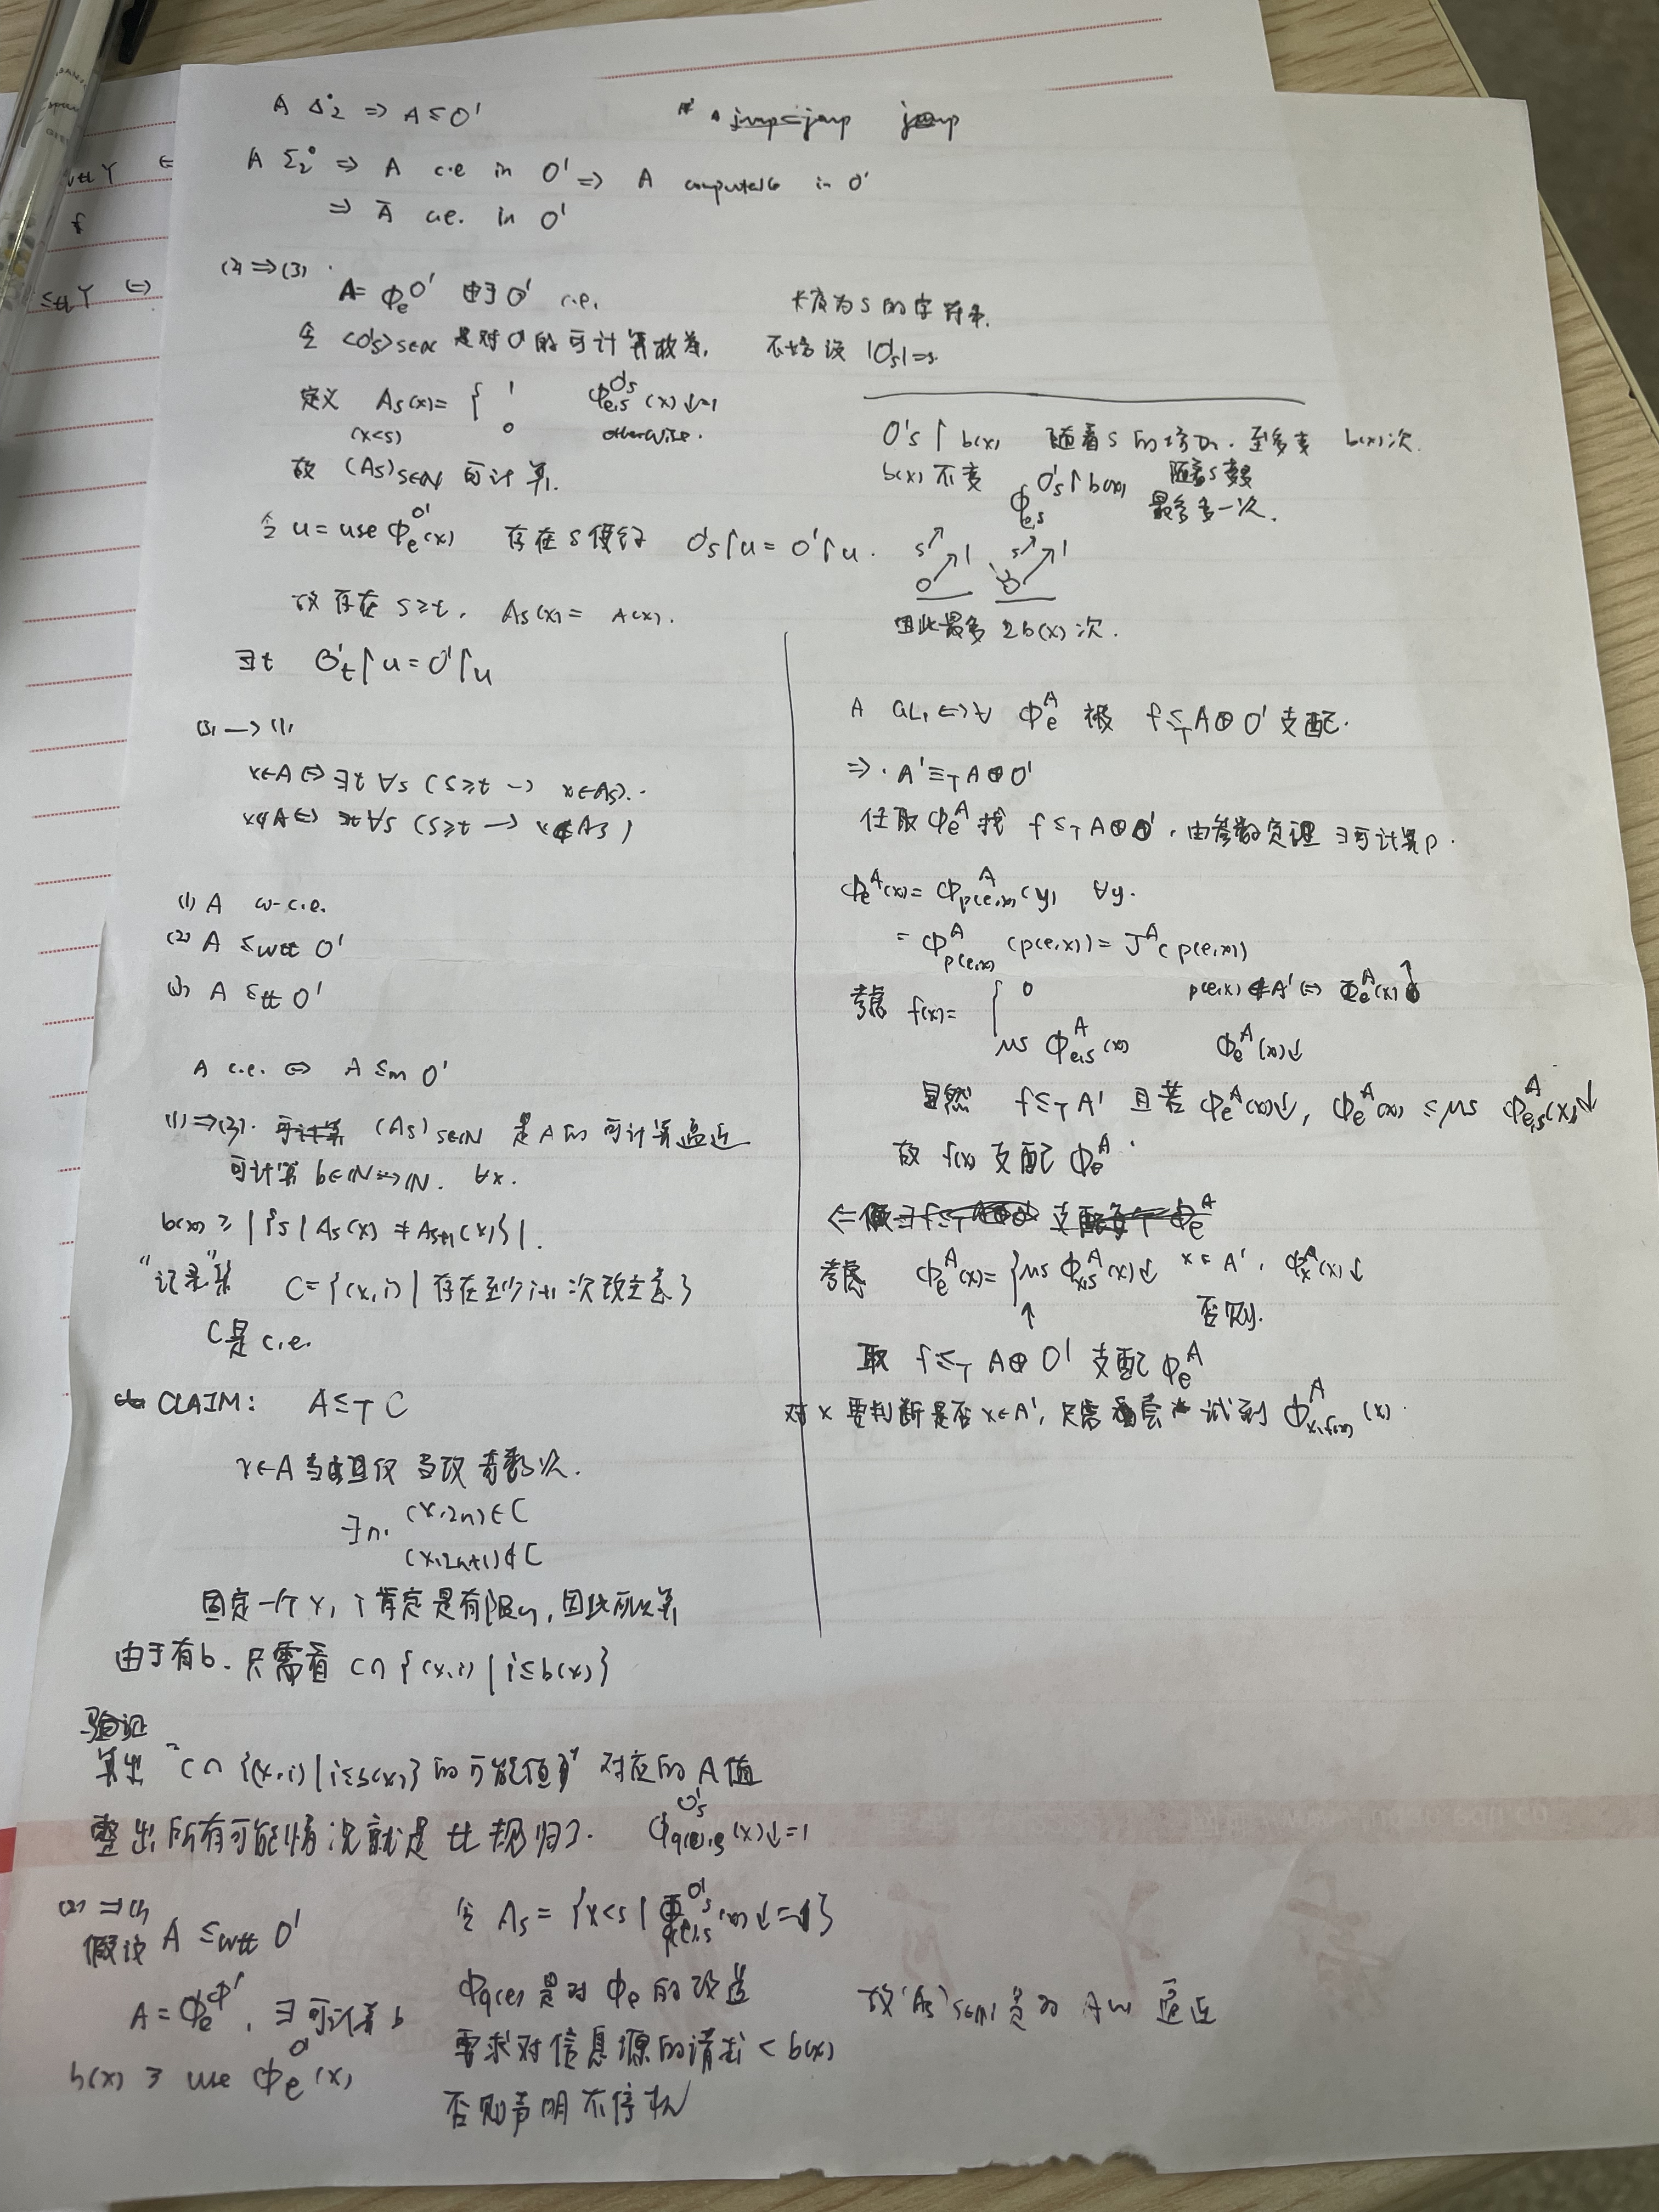
\includegraphics[width=.9\textwidth]{../images/ComputabilityAndRandomness/1.jpg}
\label{}
\end{figure}


\begin{corollary}[]
\(A\) is \(\Delta_2^0\) \(\Leftrightarrow\) \(A\) is both \(\Sigma_2^0\) and \(\Pi_2^0\)
\end{corollary}

\begin{proof}
\begin{align*}
A\in\Delta_2^0&\Leftrightarrow A\le_T\emptyset'\\
&\Leftrightarrow A\text{ and }\N-A\text{ are c.e. in }\emptyset'\\
&\Leftrightarrow A\in\Sigma_2^0\cap\Pi_2^0
\end{align*}
last iff from Theorem \ref{1.4.13}
\end{proof}


\begin{definition}[]
Let \(A\subseteq\N\) and \(n\ge 1\)
\begin{enumerate}
\item \(A\) is \(\Sigma_n^0\)if \(x\in A\leftrightarrow\exists y_1\forall y_2\dots Qy_nR(x,y_1,\dots,y_n)\), where \(R\) is a symbol for a
computable relation
\item \(A\) is \(\Pi_n^0\) if \(\N-A\) is \(\Sigma_n^0\)
\item \(A\) is \textbf{arithmetical} if \(A\) is \(\Sigma_n^0\) for some \(n\)
\end{enumerate}
\end{definition}

\begin{fact}[]
\label{1.4.12}
\(A\) is \(\Sigma_1^0\Leftrightarrow A\) is c.e.. The equivalence is uniform
\end{fact}

\begin{proof}
\(\Rightarrow\): Suppose \(x\in A\leftrightarrow\exists y R(x,y)\) for computable \(R\). Let \(\Phi\) be the partial computable
function given by the Turing program that on input \(x\) looks for a witness \(y\)
s.t. \(R(x,y)\), and halts when such a witness is found. Then \(A=\dom(\Phi)\)

\(\Leftarrow\): Suppose \(A=\dom(\Phi)\) for a partial computable function \(\Phi\). Let \(R\) be the computable
relation given by \(R(x,s)\leftrightarrow\Phi(x)[s]\downarrow\). Then \(x\in A\leftrightarrow\exists sR(x,s)\), so \(A\) is \(\Sigma_1^0\)
\end{proof}

A \(\Sigma_n^0\) set \(C\) is \textbf{\(\Sigma_n^0\)-complete} if \(A\le_mC\) for each \(\Sigma_n^0\) set \(A\)

\begin{theorem}[]
\label{1.4.13}
Let \(n\ge 1\)
\begin{enumerate}
\item \(A\) is \(\Sigma_n^0\) \(\Leftrightarrow\) \(A\) is c.e. relative to \(\emptyset^{(n-1)}\)
\item \(\emptyset^{(n)}\) is \(\Sigma_n^0\)-complete
\end{enumerate}
\end{theorem}

\begin{proof}
Induction on \(n\).  \ref{1.4.12} and \ref{1.2.2}. Now let \(n>1\)
\begin{enumerate}
\item First suppose \(A\) is \(\Sigma_n^0\) for some computable relation \(R\). Then the set
\begin{equation*}
B=\{\la x,y_1\ra:\forall y_2\dots Qy_nR(x,y_1,\dots,y_n)\}
\end{equation*}
is \(\Pi_{n-1}^0\) and \(A\) is c.e. relative to \(B\). By (2) for \(n-1\) we
have \(B\le_m\N-\emptyset^{(n-1)}\). So \(A\) is c.e. relative to \(\emptyset^{(n-1)}\)

Now suppose \(A\) is c.e. relative to \(\emptyset^{(n-1)}\). Then there is a Turing functional \(\Phi\)
s.t. \(A=\dom(\Phi^{\emptyset^{(n-1)}})\). By the use principle
\begin{equation*}
x\in A\Leftrightarrow\exists\eta,s\ucorner{\Phi_s^\eta(x)\downarrow\wedge\forall i<\abs{\eta}\;\eta(i)=1\leftrightarrow i\in\emptyset^{(n-1)}}
\end{equation*}
The innermost part can be put into \(\Sigma_n^0\)-form, so \(A\) is \(\Sigma_n^0\).
\item Follows by Proposition \ref{1.2.11} where \(Y=\emptyset^{(n-1)}\)
\end{enumerate}
\end{proof}

\begin{proposition}[]
Let \(n\ge 1\). Then \(A\) is \(\Delta_n^0\Leftrightarrow A\le_T\emptyset^{(n-1)}\)
\end{proposition}

\begin{proof}
By Theorem \ref{1.4.13}, \(A\) is \(\Delta_n^0\) \(\Leftrightarrow\) \(A\) and \(\N-A\) are c.e. in \(\emptyset^{(n-1)}\). By
Proposition \ref{1.2.8}, this condition is equivalent to \(A\le_T\emptyset^{(n-1)}\)
\end{proof}

\begin{proposition}[]
\(Z\) is \(\Sigma_2^0\) \(\Leftrightarrow\) there is a computable sequence of strong indices \((Z_s)_{s\in\N}\)
s.t. \(Z_s\subseteq[0,s)\) and \(x\in Z\leftrightarrow\exists s\forall t\ge s\;Z_t(x)=1\). The equivalence is uniform
\end{proposition}

\begin{proof}
\(\Rightarrow\): By Theorem \ref{1.4.13}, there is a Turing functional \(\Phi\) s.t. \(Z=\dom(\Phi^{\emptyset'})\). Now
let \(Z_s=\{x<s:\Phi^{\emptyset'}(x)[s]\downarrow\}\)

\(\Leftarrow\):
\end{proof}

\begin{definition}[]
The \textbf{index set} of a class \(S\) of c.e. sets is the set \(\{i:W_i\in S\}\)
\end{definition}


\begin{exercise}
\label{1.4.19}
\(\emptyset'\) is not an index set
\end{exercise}

\begin{proof}
We can find \(g\) s.t. \(W_{g(n)}=\{n\}\). Thus there is \(e\) s.t. \(W_{g(e)}=W_e=\{e\}\). By
padding lemma, we have \(W_i=W_e\) but \(i\notin\emptyset'\)
\end{proof}



\begin{exercise}
\label{1.4.20}
\begin{enumerate}
\item \(\{e:W_e\neq\emptyset\}\) is \(\Sigma_1^0\)-complete
\item The set \(\{e:W_e\text{ finite }\}\) is \(\Sigma_2^0\)-complete.
\item The set \(\Tot=\{e:\dom(\Phi_e)=\N\}=\{e:W_e=\N\}\) is \(\Pi_2^0\)-complete
\item Both \(\{e:W_e\text{ cofinite}\}\) and \(\Cop=\{e:W_e\text{ computable}\}\) are \(\Sigma_3^0\)-complete
\end{enumerate}
\end{exercise}

\begin{proof}
\begin{enumerate}
\item Given \(e\), \(\Phi_{f(n)}\) doesn't converge in \(\N-\{e\}\). And converges on \(e\)
if \(\Phi_e(e)\downarrow\). Thus \(\emptyset'\le_m\{e:W_e\neq\emptyset\}\)
\item Let \(\Fin=\{e:W_e\text{ finite}\}\). Then \(e\in\Fin\Leftrightarrow\exists s\forall t\ge s(W_{e,s}=W_{e,t})\)
\item \(e\in\Tot\Leftrightarrow\forall n\exists s\Phi_{e,s}(n)\downarrow\)

For any \(A\) in \(\Pi_2^0\), \(x\in A\Leftrightarrow\forall y\exists zR(x,y,z)\)

We could define
\begin{equation*}
\Phi_{q(x)}(u)=
\begin{cases}
0&\forall y\le u\exists zR(x,y,z)\\
\uparrow
\end{cases}
\end{equation*}
Then \(x\in A\Leftrightarrow W_{q(x)}=\omega\Leftrightarrow q(x)\in\Tot\)

\(x\in\barA\Leftrightarrow W_{q(x)}\) is finite
\item \(e\in\Cof\Leftrightarrow\exists z\forall n\ge z\exists s\Phi_{e,s}(n)\downarrow\), thus \(\Cof\in\Sigma_3^0\)

check fudan's textbook p120
\end{enumerate}
\end{proof}

\begin{exercise}
\label{1.4.21}
The set \(\{e:\dom\Phi_e^{\emptyset'}=\N\}\) is \(\Pi_0^3\)-complete
\end{exercise}

\begin{exercise}
\label{1.4.22}
Let \(\cals\) be a class of c.e. sets [\(\omega\)-c.e. sets] containing all the finite sets. Suppose the
index set of \(S\) is \(\Sigma_3^0\).  Then \(\cals\) is uniformly c.e. [uniformly c.e.]
\end{exercise}

\begin{proof}
Let \(I=\{e\mid\exists x\forall y\exists z\;R(e,x,y,.z)\}\), \(\cals=\{W_e\}_{e\in I}\)

\(\cals\) is \(\Sigma_3^0\), \(\cals\le_m\Cof\)
\end{proof}

\begin{exercise}
\label{1.4.24}
Let \(X\subseteq\N\)
\begin{enumerate}
\item Each relation \(R\le_TX\) is first-order definable in the structure \((\N,+,\cdot ,X)\)
\item The index set \(\{e:W_e\le_TX\}\) is \(\Sigma_3^0(X)\)
\end{enumerate}
\end{exercise}

\begin{proof}

\end{proof}

\begin{exercise}
\label{1.4.25}
\(A\) is \(\Delta_n^0\) \(\Leftrightarrow\) \(\forall x A(x)=\lim_{k_1}\dots\lim_{k_{n-1}}g(x,k_1,\dots,k_{n-1})\) for some
computable \(\{0,1\}\)-valued function \(g\)
\end{exercise}
\subsection{Absolute computational complexity of sets}
\label{sec:org6eb2f8c}
\subsubsection{Sets that are \texorpdfstring{\(low_n\)}{lown}}
\label{sec:orgdc0ef95}
\begin{definition}[]
Let \(f,g:\N\to\R\). \(f\) \textbf{dominates} \(g\) if \(f(n)\ge g(n)\) for almost every \(n\)
\end{definition}

\begin{enumerate}
\item \(A\) is \textbf{low} if \(A'\le_T\emptyset'\)
\item \(A\) is \textbf{computably dominated} if each function \(g\le_TA\) is dominated by a computable
function
\item \(A\) is \textbf{high} if \(\emptyset''\le_TA'\)
\end{enumerate}


\begin{definition}[]
Let \(n\ge 0\). We say that \(C\) is \(low_n\) if \(C^{(n)}\equiv_T\emptyset^{(n)}\)
\end{definition}

If \(C\in low_1\) we simply say that \(C\) is \textbf{low}. Each low set is \(\Delta_2^0\).

Each class \(low_n\) is closed downward under Turing reducibility, and contained in \(\Delta_{n+1}^0\)
\begin{equation*}
\text{computable}\subset low_1\subset low_2\subset\dots\subset\{Z:Z\not\ge_T\emptyset'\}
\end{equation*}

\begin{definition}[]
\(C\) is \textbf{superlow} if \(C'\equiv_{tt}\emptyset'\)
\end{definition}

It suffices to require that \(C'\le_{tt}\emptyset'\), because \(\emptyset'\le_mC'\) for any \(C\) by \ref{1.2.14}. By
\ref{1.4.4} it is equivalent to ask that \(C'\) be \(\omega\)-c.e.

\begin{definition}[]
\(A\) is \textbf{generalized \(low_1\)}, or in \(\GL_1\) for short, if \(A'\equiv_TA\oplus\emptyset'\)
\end{definition}

\begin{exercise}
\label{1.5.5}
If \(C\) is superlow, there is a computable function \(h\) s.t. \(Y\le_TC\) implies \(Y\le_{tt}\emptyset'\)
with use function bounded by \(h\) for each \(Y\)
\end{exercise}

\begin{proof}

\end{proof}

\begin{exercise}
\label{1.5.7}
If \(B\) is \(low_2\) then the index set \(\{e:W_e\le_TB\}\) is \(\Sigma_3^0\)
\end{exercise}

\begin{exercise}
\label{1.5.8}
\(B\) is \(low_2 \Leftrightarrow\) \(\Tot^B=\{e:\Phi_e^B\text{ total}\}\) is \(\Sigma_3^0\)
\end{exercise}
\subsubsection{Computably dominated sets}
\label{sec:orge219fd4}
\begin{definition}[]
\(A\) is called \textbf{computably dominated} if each function \(g\le_TA\) is dominated by a computable
function
\end{definition}

\(E\subseteq\N\)  is \textbf{hyperimmune} if \(E\) is infinite and \(p_E\) is not dominated by a computable
function, where \(p_E\) is the listing of \(E\) in order of magnitude

\begin{proposition}[]
\(A\) is not computably dominated \(\Leftrightarrow\) there is a hyperimmune set \(E\equiv_TA\)
\end{proposition}

\begin{proof}
\(\Leftarrow\): immediate since \(p_E\le_TE\)

\(\Rightarrow\): Suppose \(g\le_TA\) is not dominated by a computable function. Let \(E=\ran(h)\), where the
function \(h\) is defined as follows: \(h(0)=0\), and for each \(n\in\N\), \(h(2n+1)=h(2n)+g(n)+1\)
and \(h(2n+2)=h(2n+1)+p_A(n)+1\).
\end{proof}

\begin{proposition}[]
\(A\) is computably dominated \(\Leftrightarrow\) for each function \(f\)
\begin{equation*}
f\le_TA\to f\le_{tt}A
\end{equation*}
\end{proposition}

\begin{proof}
\(\Rightarrow\): Suppose \(f=\Phi^A\). Let \(g(x)=\mu s\Phi_s^A(x)\downarrow\). Then \(g\le_TA\), so there is a computable
function \(t\) s.t. \(t(x)\ge g(x)\) for each \(x\). Thus \(t\) bounds the running time of \(\Phi^A\),
whence \(f\le_{tt}A\) by Proposition \ref{1.2.22}
\end{proof}

\begin{proposition}[]
If \(A\) is \(\Delta_2^0\) and incomputable, then \(A\) is not computably dominated
\end{proposition}

\begin{proof}
Let \((A_s)_{s\in\N}\) be a computable approximation of \(A\). Then the following function \(g\) is
total
\begin{equation*}
g(s)\simeq\mu t\ge s.A_t\uhr s=A\uhr s
\end{equation*}
Note that \(g\le_TA\). Assume that there is a computable function \(f\) s.t. \(g(s)\le f(s)\) for
each \(s\). Then \(A\) is computable: for each \(n\) and each \(s>n\) we have \(A_t(n)=A(n)\)
for some \(t\in[s,f(s))\), namely \(t=g(s)\). On the other hand, if \(s\) is sufficiently large
then \(A_u(n)=A_s(n)\) for all \(u\ge s\). Thus to compute \(A\), on input \(n\) determine the
least \(s>n\) s.t. \(A_u(n)=A_s(n)\) for all \(u\in[s,f(s))\). Then \(A_s(n)=A(n)\), so the
output \(A_s(n)\) is correct
\end{proof}
\subsubsection{Sets that are \texorpdfstring{\(high_n\)}{highn}}
\label{sec:org2c27c16}
\begin{definition}[]
Let \(n\ge 0\). A set \(C\) is \(high_n\) if \(\emptyset^{(n+1)}\le_TC^{(n)}\)
\end{definition}

All the classes \(high_n\) are closed upward under Turing reducibility, so the complementary
classes \(\non-high_n=2^{\N}-high_n\) are closed downward. Therefore
\begin{equation*}
comp.\subset low_1\subset low_2\subset\dots\subset\non-high_2\subset\non-high_1\subset\{Z:Z\not\ge_T\emptyset'\}
\end{equation*}

It is easy to define a function \(f\le_T\emptyset'\) that dominates all computable functions: the
set \(\{\la e,x\ra:\Phi_e(x)\downarrow\}\) is c.e., and hence many-one reducible to \(\emptyset'\) via a computable
function \(h\). Let \(f(x)=\max\{\Phi_e(x):e\le x\wedge h(\la e,x\ra)\in\emptyset')\}\). If \(\Phi_e\) is total
then \(f(x)\ge\Phi_e(x)\) for all \(x\ge e\). This property of \(\emptyset'\) in fact characterizes the high
sets.

\begin{theorem}[]
\(C\) is high \(\Leftrightarrow\) some function \(f\le_TC\) dominates all computable functions
\end{theorem}

\begin{proof}
\(\Rightarrow\): We define a function \(f\le_TC\) that dominates each total \(\Phi_e\), extending the argument
for the case \(C=\emptyset'\). Note that \(\Tot=\{e:\Phi_e\text{ total}\}\) is \(\Pi_2^0\), and
hence \(\ove{\Tot}\le_m\emptyset''\le_TC'\). By the Limit Lemma \ref{1.4.2}, \(\Tot\) is \(\Delta_2^0(C)\), there is
a binary function \(p\le_TC\) s.t. for each \(e\), \(\lim_sp(e,s)\) exists and \(\lim_sp(e,s)=1\)
iff \(\Phi_e\) is total
\end{proof}
\end{document}
